\chapter{Analysis}
\label{chapter:analysis}

Now we investigate the proposed system, which is in general intractable, but will provide motivation for future developments.

\section{Mathematical Investigation}
\label{section:mathematical development}
This section is an investigation into the initial three frames\footnote{Technically, two frames. Frame 1, $\pmb{x}_0$, can be absorbed and then ignored.} of the system. Figure~\ref{figure:identity_resolved} provides a useful analogue of what is happening in the initial frames, but it is the same for far too many reasons (mainly because drawing joint distributions in TIKZ is difficult). 
\begin{figure}[!ht]
    \centering
    \begin{subfigure}[t]{0.5\textwidth}
        \centering
        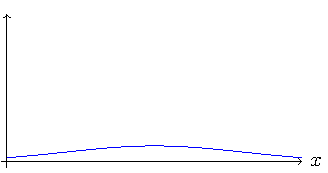
\includegraphics[height=3.5cm]{tikz/prior}
        \caption{As always, we initially know nothing about state $x_1^{1}$.}
    \end{subfigure}%
    ~
    \begin{subfigure}[t]{0.5\textwidth}
        \centering
        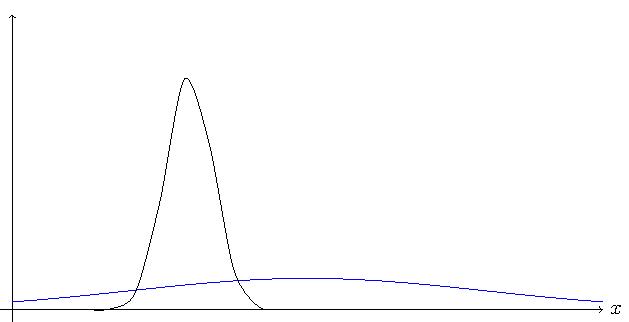
\includegraphics[height=3.5cm]{tikz/prior_measurement}
        \caption{The belief is updated with a specific measurement, the object now has a stronger association with a specific trajectory.}
    \end{subfigure}%
    
    \centering
    \begin{subfigure}[t]{0.5\textwidth}
        \centering
        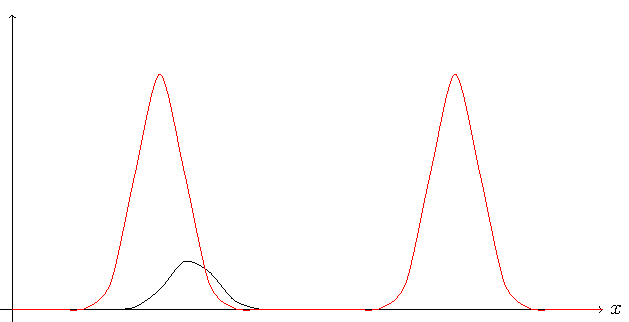
\includegraphics[height=3.5cm]{tikz/measurement_product}
        \caption{Before the measurement update of $x_2^1$. The measurement update will always think both measurements were likely to been caused by $x_1$.}
    \end{subfigure}%
   ~
    \centering
    \begin{subfigure}[t]{0.5\textwidth}
        \centering
        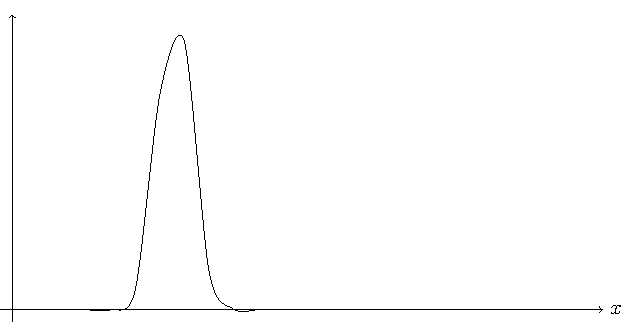
\includegraphics[height=3.5cm]{tikz/second_mixture_product}
        \caption{After the measurement update, the trajectory associated with $x_1$ dominates, though this is technically still a mixture of Gaussians. }
    \end{subfigure}%    
    \caption{A system analogous to that developed in the Chapter~\ref{chapter:representation}. The distribution of $x_{t}^{1}$ is a Gaussian mixture with an exponential amount of components, a component for every possible trajectory introduced by the measurement update. This approach primes the system so that a target's state is strongly associated with a specific trajectory. }
    \label{figure:identity_resolved}
\end{figure}

\subsection{The Measurement Message}
\label{subsection:measurement_message}
All measurement distributions have the same form:
\begin{align}
\pmb{C}_{\pmb{z} \left( t \right)} \left( \pmb{x}_{t}^{1},  \pmb{x}_{t}^{2}, \pmb{z}_{t}^{1},  \pmb{z}_{t}^{2}, a_{t} \right) 
&= \begin{cases}
 \mathcal{N}\left( \pmb{z}_{t}^{1} | C \pmb{x}_{t}^{1}, Q \right)  \mathcal{N}\left( \pmb{z}_{t}^{2} | C \pmb{x}_{t}^{2}, Q \right)  \mbox{if} \ a_{t} = 1 \\
 \mathcal{N}\left( \pmb{z}_{t}^{1} | C \pmb{x}_{t}^{2}, Q \right)  \mathcal{N}\left( \pmb{z}_{t}^{2} | C \pmb{x}_{t}^{1}, Q \right)  \mbox{if} \ a_{t} = 2 
\end{cases} \\
&= \begin{cases}
 \mathcal{C}\left( \pmb{x}_{t}^{1}, \pmb{z}_{t}^{1}; \hat{P}, \pmb{0}, \hat{g}  \right) \mathcal{C}\left( \pmb{x}_{t}^{2}, \pmb{z}_{t}^{2}; \hat{P}, \pmb{0}, \hat{g}  \right) \mbox{if} \ a_{t} = 1 \\
 \mathcal{C}\left( \pmb{x}_{t}^{1}, \pmb{z}_{t}^{2}; \hat{P}, \pmb{0}, \hat{g}  \right) \mathcal{C}\left( \pmb{x}_{t}^{2}, \pmb{z}_{t}^{1}; \hat{P}, \pmb{0}, \hat{g}  \right)  \mbox{if} \ a_{t} = 2 
\end{cases}
\end{align}
Where,
\begin{align}
\hat{P} &= \begin{bmatrix}
C^{T} Q^{-1} C & -C^{T} Q^{-1} \\ 
-Q^{-1} C & Q^{-1} 
\end{bmatrix} \\
\hat{g} &= - \ln \left( \left( 2 \pi \right)^{k/2} | Q |^{1/2} \right)
\end{align}
The measurement update message, after observing $\pmb{z}_{t}^{1}$ and $\pmb{z}_{t}^{2}$:
\begin{align*}
\delta_{\pmb{z}(t) \rightarrow \pmb{x}(t)} \left( \pmb{x}_{t}^{1}, \pmb{x}_{t}^{2} \right)  &= \int \pmb{C}_{\pmb{z} \left( t \right)} \left( \pmb{x}_{t}^{1},  \pmb{x}_{t}^{2}, \pmb{z}_{t}^{1} = \pmb{z}_{t}^{2},  \pmb{z}_{t}^{2} = \pmb{z}_{t}^{2}, a_{t} \right) d \{ a_{t} \} \\
&= \frac{1}{2} \mathcal{C} \left(  \pmb{x}_{t}^{1},  \pmb{x}_{t}^{2}; P_{\pmb{z}}  ,  \pmb{h}_{\pmb{z}(1)}, g_{\pmb{z}} \right) + \frac{1}{2} \mathcal{C} \left(  \pmb{x}_{t}^{1},  \pmb{x}_{t}^{2}; P_{\pmb{z}}, \pmb{h}_{\pmb{z}(2)}, g_{\pmb{z}} \right) \numberthis
\end{align*}
This a two component Gaussian mixture, where:
\begin{align}
P_{\pmb{z}} &= \begin{bmatrix}
C^{T} Q^{-1} C & 0 \\
0 & C^{T} Q^{-1} C 
\end{bmatrix} \\
\pmb{h}_{\pmb{z}(1)} &=  \begin{bmatrix}
C^{T} Q^{-1} \pmb{z}_{t}^{1} \\
C^{T} Q^{-1} \pmb{z}_{t}^{2} 
\end{bmatrix} \\
\pmb{h}_{\pmb{z}(1)} &=  \begin{bmatrix}
C^{T} Q^{-1} \pmb{z}_{t}^{2} \\
C^{T} Q^{-1} \pmb{z}_{t}^{1} 
\end{bmatrix} \\
g_{\pmb{z}} &= - \ln \left( \left( 2 \pi \right)^{k} | Q | \right) - \frac{1}{2} (\pmb{z}_{t}^{1})^{T} Q^{-1} (\pmb{z}_{t}^{1}) - \frac{1}{2} (\pmb{z}_{t}^{2})^{T} Q^{-1} (\pmb{z}_{t}^{2})
\end{align}

\subsection{Recursive Belief Message}
\label{subsection:recursive_belief}
At time step $t=1$ the system is simply the product of two independent Kalman Filters. Rather than formal derivation, its easier just to propagate a Gaussian forward using the standard Kalman Filter equations:
\begin{align*}
\therefore \delta_{\pmb{x}(1) \rightarrow \pmb{x}(2)} \left( \pmb{x}_{1}^{1}, \pmb{x}_{1}^{2} \right)  &= \int \pmb{C}_{\pmb{x} \left( 1 \right)} \left( \pmb{x}_{0}^{1},  \pmb{x}_{0}^{2}, \pmb{x}_{1}^{1},  \pmb{x}_{1}^{2} \right) d\{ \pmb{x}_{0}^{1},  \pmb{x}_{0}^{2} \} \\
&= \mathcal{C} \left( \pmb{x}_{1}^{1}, \pmb{x}_{1}^{2}; P_{\pmb{x}(1)}, \pmb{h}_{\pmb{x}(1)}, g_{\pmb{x}(1)} \right) \numberthis
\end{align*}
Where,
\begin{align*}
P_{\pmb{x}(1)} &= \begin{bmatrix}
\left( \Sigma_{1}^{1} \right)^{-1} & 0 \\
0 & \left( \Sigma_{1}^{2} \right)^{-1} 
\end{bmatrix} \numberthis \\
\pmb{h}_{\pmb{x}(1)} &= \begin{bmatrix}
\left( \Sigma_{1}^{1} \right)^{-1} \pmb{\mu}_{1}^{1} \\
\left( \Sigma_{1}^{2} \right)^{-1} \pmb{\mu}_{1}^{2} 
\end{bmatrix} \numberthis \\
g_{\pmb{x}(1)} &= - \ln \left( \left( 2 \pi \right)^{n/2} | \Sigma_{1}^{1} |^{1/2} \right) - \ln \left( \left( 2 \pi \right)^{n/2} | \Sigma_{1}^{2} |^{1/2} \right) \\
&- \frac{1}{2} (\pmb{\mu}_{1}^{1})^{T} \left( \Sigma_{1}^{1} \right)^{-1} (\pmb{\mu}_{1}^{1}) - \frac{1}{2} (\pmb{\mu}_{1}^{2})^{T} \left( \Sigma_{1}^{2} \right)^{-1} (\pmb{\mu}_{1}^{2}) \numberthis
\end{align*}
I never derived the scalar $g_{\pmb{x}(t)}$ last time and most people seem to ignore it, but the outgoing message is Gaussian so $g_{\pmb{x}(t)}$ should be valid.

\subsection{The Second Frame}
\label{subsection:the_second_frame}
Before any updates occur, the following uninformed potential inhabits $\pmb{C}_{\pmb{x}(2)}$:
\begin{align*}
\pmb{C}_{\pmb{x} \left( 2 \right)} \left( \pmb{x}_{1}^{1},  \pmb{x}_{1}^{2}, \pmb{x}_{2}^{1},  \pmb{x}_{2}^{2} \right) &=  \mathcal{C}_{\pmb{x}(2)} \left( \pmb{x}_{1}^{1},  \pmb{x}_{2}^{1} ,  \pmb{x}_{1}^{2} ,  \pmb{x}_{2}^{2} ; P_{\pmb{x}(2)}, \pmb{h}_{\pmb{x}(2)}, g_{\pmb{x}(2)}   \right) \\
\end{align*}
Where,
\begin{align}
P_{\pmb{x}(2)} &= \begin{bmatrix}
\begin{matrix} R^{-1} & -R^{-1} A \\ -A^{T} R^{-1} & A^{T} R^{-1} A \end{matrix} & \begin{matrix} 0 \end{matrix} \\
\begin{matrix} 0 \end{matrix} & \begin{matrix} R^{-1} & -R^{-1} A \\ -A^{T} R^{-1} & A^{T} R^{-1} A \end{matrix}
\end{bmatrix} \\
\pmb{h}_{\pmb{x}(2)} &= \begin{bmatrix}
R^{-1} B \pmb{u} \\
-A R^{-1} B \pmb{u} \\
R^{-1} B \pmb{u} \\
-A R^{-1} B \pmb{u} 
\end{bmatrix} \\
g_{\pmb{x}(2)} &= -\ln( (2\pi)^{n} | R | ) - \frac{1}{2} \pmb{h}_{\pmb{x}(2)}^{T} P_{\pmb{x}(2)}^{-1} \pmb{h}_{\pmb{x}(2)}
\end{align}
\subsubsection{Belief Update}
\label{section:belief_update}
The outgoing message from $\pmb{C}_{\pmb{x}(2)}$:
\begin{align*}
\delta_{\pmb{x}(2) \rightarrow \pmb{x}(3)} \left( \pmb{x}_{2}^{1}, \pmb{x}_{2}^{2} \right) &= \delta_{\pmb{z}(2) \rightarrow \pmb{x}(3)} \left( \pmb{x}_{2}^{1}, \pmb{x}_{2}^{2} \right) \underbrace{ \int \pmb{C}_{\pmb{x} \left( 2 \right)} \left( \pmb{x}_{1}^{1},  \pmb{x}_{1}^{2}, \pmb{x}_{2}^{1},  \pmb{x}_{2}^{2} \right)  \delta_{\pmb{x}(1) \rightarrow \pmb{x}(2)} \left( \pmb{x}_{1}^{1}, \pmb{x}_{1}^{2} \right) d\{ \pmb{x}_{1}^{1}, \pmb{x}_{1}^{2} \} }_{\Psi \left( \pmb{x}_{1}^{1}, \pmb{x}_{1}^{2} \right)}
\end{align*}
$\Psi \left( \pmb{x}_{1}^{1}, \pmb{x}_{1}^{2} \right)$ is nothing new, the established equations just have to be applied independently. Giving:
\begin{align}
\Psi \left( \pmb{x}_{1}^{1}, \pmb{x}_{1}^{2} \right) &= \mathcal{C} \left( \pmb{x}_{2}^{1}, \pmb{x}_{2}^{2}; P_{\Psi}, \pmb{h}_{\Psi}, g_{\Psi} \right)
\end{align}
Where,
\begin{align*}
P_{\Psi} &= \begin{bmatrix}
\left( R + A \Sigma_{1}^{1} A^{T} \right)^{-1} & 0 \\
0 & \left( R + A \Sigma_{1}^{2} A^{T} \right)^{-1} \\
\end{bmatrix} \\
&= \begin{bmatrix}
\left( \overline{\Sigma}_{2}^{1} \right)^{-1} & 0 \\
0 & \left( \overline{\Sigma}_{2}^{2} \right)^{-1} \\
\end{bmatrix} \numberthis \\
\pmb{h}_{\Psi} &= \begin{bmatrix}
\left( R + A \Sigma_{1}^{1} A^{T} \right)^{-1} ( A \pmb{\mu}_{1}^{1} + B \pmb{u} ) \\
\left( R + A \Sigma_{1}^{2} A^{T} \right)^{-1} ( A \pmb{\mu}_{1}^{2} + B \pmb{u} )
\end{bmatrix} \\
&= \begin{bmatrix}
\left( \overline{\Sigma}_{2}^{1} \right)^{-1}  \overline{\pmb{\mu}}_{2}^{1}  \\
\left( \overline{\Sigma}_{2}^{1} \right)^{-1}  \overline{\pmb{\mu}}_{2}^{2}  
\end{bmatrix} \numberthis \\
g_{\Psi} &=  -\ln( (2\pi)^{n/2} | R + A \Sigma_{1}^{1} A^{T} |^{1/2} ) -\ln( (2\pi)^{n/2} | R + A \Sigma_{1}^{1} A^{T} |^{1/2} ) \nonumber \\
&- \frac{1}{2} \pmb{h}_{\Psi}^{T} P_{\Psi}^{-1} \pmb{h}_{\Psi} \numberthis
\end{align*}
$g_{\Psi}$ is not necessarily correct, but I really hate dealing with it, so I'm not going to.

\subsubsection{Measurement Update}
\label{subsubsection:measurement_update}
Eventually, 
\begin{align*}
\delta_{\pmb{x}(2) \rightarrow \pmb{x}(3)} \left( \pmb{x}_{2}^{1}, \pmb{x}_{2}^{2} \right)  &= \delta_{\pmb{z}(2) \rightarrow \pmb{x}(2)} \left( \pmb{x}_{2}^{1}, \pmb{x}_{2}^{2} \right) \Psi \left( \pmb{x}_{1}^{1}, \pmb{x}_{1}^{2} \right) \\
&= \mathcal{C} \left( \pmb{x}_{2}^{1}, \pmb{x}_{2}^{2}; P_{\pmb{z}(2)}, h_{\pmb{z}(2)}, g_{\pmb{z}(2)} \right) \mathcal{C} \left( \pmb{x}_{2}^{1}, \pmb{x}_{2}^{2}; P_{\Psi}, \pmb{h}_{\Psi}, g_{\Psi} \right) \\
&= \frac{1}{2} \mathcal{C} \left(  \pmb{x}_{2}^{1},  \pmb{x}_{2}^{2}; P_{\pmb{z}}  ,  \pmb{h}_{\pmb{z}(1)}, g_{\pmb{z}} \right) \mathcal{C} \left( \pmb{x}_{2}^{1}, \pmb{x}_{2}^{2}; P_{\Psi}, \pmb{h}_{\Psi}, g_{\Psi} \right) \\
&+ \frac{1}{2} \mathcal{C} \left(  \pmb{x}_{2}^{1},  \pmb{x}_{2}^{2}; P_{\pmb{z}}, \pmb{h}_{\pmb{z}(2)}, g_{\pmb{z}} \right) \mathcal{C} \left( \pmb{x}_{2}^{1}, \pmb{x}_{2}^{2}; P_{\Psi}, \pmb{h}_{\Psi}, g_{\Psi} \right)  \\
&= \frac{1}{2} \mathcal{C} \left(  \pmb{x}_{2}^{1},  \pmb{x}_{2}^{2}; P_{\pmb{x}(2)}  ,  \pmb{h}_{\pmb{x}(2)}^{1}, g_{\pmb{x}(2)} \right) + \frac{1}{2} \mathcal{C} \left(  \pmb{x}_{2}^{1},  \pmb{x}_{2}^{2}; P_{\pmb{x}(2)} , \pmb{h}_{\pmb{z}(2)}^{2}, g_{\pmb{x}(2)} \right)
\end{align*}
Where,
\begin{align}
P_{\pmb{x}(2)} &= \begin{bmatrix}
\left( \overline{\Sigma}_{2}^{1} \right)^{-1} + C^{T} Q^{-1} C & 0 \\
0 & \left( \overline{\Sigma}_{2}^{2} \right)^{-1} + C^{T} Q^{-1} C 
\end{bmatrix} \\
\pmb{h}_{\pmb{x}(2)}^{1} &= \begin{bmatrix}
C^{T} Q^{-1} \pmb{z}_{2}^{1} + \left( \overline{\Sigma}_{2}^{1} \right)^{-1} \overline{\pmb{\mu}}_{2}^{1} \\
C^{T} Q^{-1} \pmb{z}_{2}^{2} + \left( \overline{\Sigma}_{2}^{2} \right)^{-1} \overline{\pmb{\mu}}_{2}^{2} \\
\end{bmatrix} \\
\pmb{h}_{\pmb{x}(2)}^{2} &= \begin{bmatrix}
C^{T} Q^{-1} \pmb{z}_{2}^{2} + \left( \overline{\Sigma}_{2}^{1} \right)^{-1} \overline{\pmb{\mu}}_{2}^{1} \\
C^{T} Q^{-1} \pmb{z}_{2}^{1} + \left( \overline{\Sigma}_{2}^{2} \right)^{-1} \overline{\pmb{\mu}}_{2}^{2} \\
\end{bmatrix} 
\end{align}
From this,
\begin{align*}
\Sigma_{\pmb{x}(2)} &= \begin{bmatrix}
\left( I - K_{2}^{1} C \right) \overline{\Sigma}_{2}^{1} & 0 \\
0 & \left( I - K_{2}^{2} C \right) \overline{\Sigma}_{2}^{2} \\
\end{bmatrix} \numberthis \\
\pmb{\mu}_{\pmb{x}(2)}^{1} &= P_{\pmb{x}(2)}  \pmb{h}_{\pmb{x}(2)}^{1} \\
&= \begin{bmatrix}
\overline{\pmb{\mu}}_{2}^{1} + K_{1}^{1} \left( \overline{\pmb{\mu}}_{2}^{1} - C \pmb{z}_{2}^{1} \right) \\
\overline{\pmb{\mu}}_{2}^{2} + K_{1}^{2} \left( \overline{\pmb{\mu}}_{2}^{2} - C \pmb{z}_{2}^{2} \right)
\end{bmatrix} \\
\pmb{\mu}_{\pmb{x}(2)}^{2} &= P_{\pmb{x}(2)}  \pmb{h}_{\pmb{x}(2)}^{2} \\
&= \begin{bmatrix}
\overline{\pmb{\mu}}_{2}^{1} + K_{1}^{1} \left( \overline{\pmb{\mu}}_{2}^{1} - C \pmb{z}_{2}^{2} \right) \\
\overline{\pmb{\mu}}_{2}^{2} + K_{1}^{2} \left( \overline{\pmb{\mu}}_{2}^{2} - C \pmb{z}_{2}^{1} \right)
\end{bmatrix}
\end{align*}
This is all good and well, but its difficult to see the state of a single target from the joint representation. Looking at just $\pmb{x}_{2}^{1}$: 
\begin{align}
\Phi \left( \pmb{x}_{2}^{1} \right) &= \int \delta_{\pmb{x}(2) \rightarrow \pmb{x}(3)} \left( \pmb{x}_{2}^{1}, \pmb{x}_{2}^{2} \right) d \pmb{x}_{2}^{2} \nonumber \\
&= \frac{1}{2} \mathcal{C} \left(  \pmb{x}_{2}^{1}; P_{\pmb{x}}  ,  \pmb{h}_{\pmb{x}}^{1}, g_{\pmb{x}} \right) + \frac{1}{2} \mathcal{C} \left(  \pmb{x}_{2}^{1}; P_{\pmb{x}}  ,  \pmb{h}_{\pmb{x}}^{2}, g_{\pmb{x}} \right)
\end{align}
Where,
\begin{align}
P_{\pmb{x}} &= C^{T} Q^{-1} \pmb{z}_{2}^{1} + \left( \overline{\Sigma}_{2}^{1} \right)^{-1} \overline{\pmb{\mu}}_{2}^{1} \\
\pmb{h}_{\pmb{x}}^{1} &= C^{T} Q^{-1} \pmb{z}_{2}^{1} + \left( \overline{\Sigma}_{2}^{1} \right)^{-1} \overline{\pmb{\mu}}_{2}^{1} \\
\pmb{h}_{\pmb{x}}^{2} &= C^{T} Q^{-1} \pmb{z}_{2}^{2} + \left( \overline{\Sigma}_{2}^{2} \right)^{-1} \overline{\pmb{\mu}}_{2}^{2} 
\end{align}
Now,
\begin{align}
\Sigma_{\pmb{x}(2)}&= \left( I - K_{1}^{1} C \right) \overline{\Sigma}_{1}^{1} \\
\pmb{\mu}_{\pmb{x}(2)}^{1} &= \overline{\pmb{\mu}}_{2}^{1} + K_{1}^{1} \left( \overline{\pmb{\mu}}_{2}^{1} - C \pmb{z}_{2}^{1} \right) \\
\pmb{\mu}_{\pmb{x}(2)}^{2} &= \overline{\pmb{\mu}}_{2}^{1} + K_{1}^{1} \left( \overline{\pmb{\mu}}_{2}^{1} - C \pmb{z}_{2}^{2} \right) 
\end{align}
From this representation it can be seen we are essentially running two Kalman Filters in parallel. The will system pursue both possible trajectories introduced by the measurement update. Although this system is set-up to ensure one trajectory will dominate, see Figure~\ref{figure:identity_resolved}.

\subsection{And Beyond \dots}
\label{subsection:beyond}
We have now established, with some rigour (except for $g$), that from time steps $t>2$ a mixture of Gaussians is being propagated forwards in time. After each measurement update the number of mixture components double, for a time step $n$ there are $T(n) = 2^{n-1}$ many mixture components. The system is similar to running exponential number of Kalman Filters in parallel, each pursuing the possible trajectories the measurement updates imply. Naturally, most components will decay after time, but they will still be present in the mixture.

Figure~\ref{figure:binary_tree} shows the exponential explosion of mixture components for $n$ time steps. Each of the leaves is a mixture component with its measured trajectory being the path back to the root. The red path is the dominant mixture component.
\begin{figure}[!ht]
	\centering
	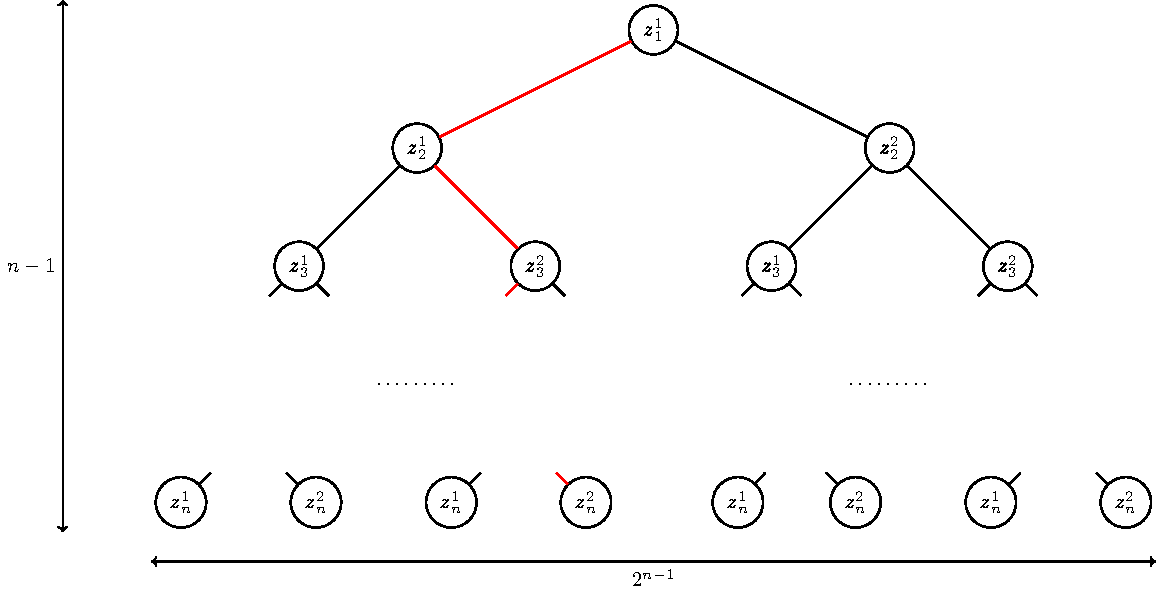
\includegraphics[scale=0.625]{tikz/binary_tree}
	\caption[An enumeration of all possible trajectories.]{A tree enumerating all possible trajectories introduced by measurement updates for $n$-many time steps. The red path is the dominant trajectory.}
	\label{figure:binary_tree}
\end{figure}

\section{Identifiability}
\label{section:identifiability}
This section is an aside which looks at the previous representation and its identity crisis. Figure~\ref{section:identifiability} shows that if we do not initially assign a specific measurement to a target, both will have significant presence in the initial mixture. Since the motion model is the same for both targets the problem becomes symmetrical and $\pmb{x}_{t}^{1}$ will be indistinguishable from $\pmb{x}_{t}^{2}$. Both mixtures will have two dominant components corresponding to the Kalman Filter's independent estimate of both targets' states, but we will not be able determine which state corresponds to which target. This approach won't have any more mixture components than Figure~\ref{figure:binary_tree}, just two dominant components.

\begin{figure}
    \centering
    \begin{subfigure}[t]{0.5\textwidth}
        \centering
        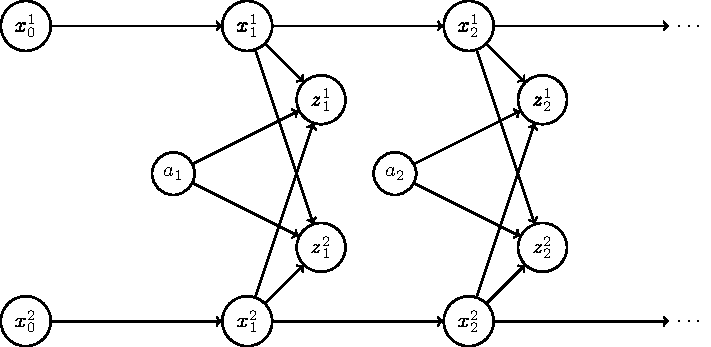
\includegraphics[height=3.5cm]{tikz/bayes_symmetrical}
        \caption{A similar system, which begins with an association problem.}
    \end{subfigure}%   
  	~
    \centering
    \begin{subfigure}[t]{0.5\textwidth}
        \centering
        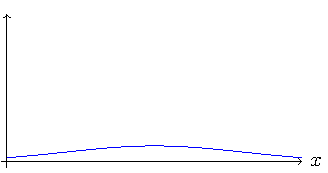
\includegraphics[height=3.5cm]{tikz/prior}
        \caption{The initial belief of $x_{1}^{1}$, we don't know much about anything.}
    \end{subfigure}%
    
    \begin{subfigure}[t]{0.5\textwidth}
        \centering
        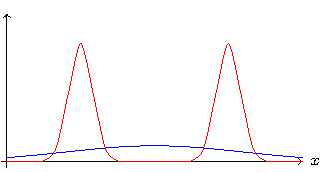
\includegraphics[height=3.5cm]{tikz/gaussian_mixture}
        \caption{Before measurement update. Both measurements are likely to been caused by $x_1^1$.}
    \end{subfigure}%
    ~
    \centering
    \begin{subfigure}[t]{0.5\textwidth}
        \centering
        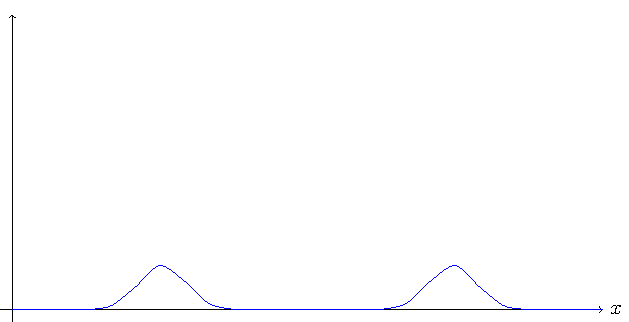
\includegraphics[height=3.5cm]{tikz/product_mixture}
        \caption{After the measurement update. Without more specific knowledge about  $x_1^{1}$'s  state, both trajectories are likely.}
    \end{subfigure}%
    \caption{An similar system with an identifiability issue. Without specific knowledge of $x_0^1$ both measurements seem likely and the state of $x_{t}^{i}$ will have two dominant components.}
    \label{figure:indentity_issue}
\end{figure}